% This is samplepaper.tex, a sample chapter demonstrating the
% LLNCS macro package for Springer Computer Science proceedings;
% Version 2.20 of 2017/10/04
%
\documentclass[runningheads]{llncs}
%
\usepackage{graphicx}
\usepackage{amsmath}
% Used for displaying a sample figure. If possible, figure files should
% be included in EPS format.
%
% If you use the hyperref package, please uncomment the following line
% to display URLs in blue roman font according to Springer's eBook style:
% \renewcommand\UrlFont{\color{blue}\rmfamily}

\begin{document}
%
\title{A Study of Cuckoo Hashing}
%
%\titlerunning{Abbreviated paper title}
% If the paper title is too long for the running head, you can set
% an abbreviated paper title here
%
\author{Zhijia Chen}

\maketitle              % typeset the header of the contribution
%
\begin{abstract}
The abstract should briefly summarize the contents of the paper in
150--250 words.

\keywords{First keyword  \and Second keyword \and Another keyword.}
\end{abstract}
%
%
%
\section{Introduction}
Some people say that the data are to this century what oil was to the last one: a driving force of growth and change. Indeed, data has been acting as fuels for many techniques such as machine learning , the Internet of Things and big data analysis, which in turn promote people to generate even more data. The data in last few decades has been growing exponentially and is supposed to keep the exploding trend. According to the report of International Data Corporation (IDC) published in 2014, the total size of data in the digital universe will reach to 44 zettabytes by 2020, and nearly 50\% of cloud-based services will rely on data in storage systems. What's more, many computing devices, from small IoT sensors to powerful server in large scale data centers, are collecting and analyzing ever-greater amounts of data. A users in routine generate queries on hundreds of Gigabytes of data stored in their local storage or cloud storage systems, and commercial companies generally handle Terabytes and even Petabytes of data each day[SmartCuckoo].

Thus it is more and more challenging for cloud storage systems to serve queries in a real-time manner and keep a stable throughput over time, which consumes substantial resources to support query-related operations[]. And effective hashing scheme is becoming a critical factor for query service to keep up with the data growth. A hash table maps a keys to values and it uses a hash function to compute the position in the table where the corresponding data could be stored or found. Hash tables are so adorable for data indexing because they have a constant lookup complexity on average which supports fast query response whatever the data size is. But hash table has also has its drawback --- hashing collision. Because a hash function usually maps multiple distinctive elements into one element, it may points multiple different keys to the same slot.

Thus one of the most basic tasks when designing a hashing scheme is to handle hashing collision.

Generally there are three strategies for resolving hashing collisions[]:

\paragraph{\textbf{Perfect hashing:}} Choose a hash function with no collisions. The idea idea of using hashing functions that prevent the collisions seems appealing. However, it requires complete knowledge of all the keys to construct a perfect hashing function[fundamental study perfect hashing], which is not feasible for large cloud data storage centers that need to handle new coming data all the time.

\paragraph{\textbf{Open addressing:}} Allow items to overflow out of their target bucket and into other paces. With open addressing, data collisions are resolved by finding alternative locations in hash table by probing a sequence of possible indices. Suppose $T_i$ is the $i$th probing position and $h(x), h_1(x), h_2(x)$ are hash functions, three basic probing methods are listed below.
\begin{itemize}
    \item Linear probing: $T_i(x)=h(x)+i$
    \item Quadratic probing: $T_i(x)=h(x)+i^2$
    \item Double hashing: $T_i(x)=h_1(x)+i\times h_2(x)$
\end{itemize}

\paragraph{\textbf{Closed addressing (separate chaining):}} All the colliding items should be stored in the target bucket with the help of some auxiliary data structures. The closed addressing (also called separate chaining) resolves hashing collision by storing all colliding items in an auxiliary linked list or BST. The basic implementation are simple, but its performance is sensitive to data distribution, as a lookup in a bucket with collisions will involve a searching the auxiliary data structure, which could be very expensive in some unfortunate cases where too much keys are collided in the bucket due to skewed distribution of data.\\

Both open addressing and closed addressing, however, will suffer from great latencies when there are too many collisions in the target bucket under some unfortunate cases. So people are looking for hashing schemes that could have a constant lookup time even in the worst case, and cuckoo hashing is one of those candidates. Cuckoo hashing is a fast and simple hashing scheme with constant-time worst-case lookup ($O(ln\frac{1}{\epsilon})$) and has $(1+\epsilon)n$ memory consumption, where $\epsilon$ is a small constant. It is widely used in large storage systems for its desirable properties. Unlike simple hashing schemes that provide only one bucket, cuckoo hashing provides $N$ ($N=2$ in common practice) possible locations for each item by using $N$ hash functions to reduce the change of collision. And to resolve collisions, old items are kicked out by the new comers and turn to their alternate buckets. To look up for an item, the cuckoo hashing only needs to search for a small number of buckets (depends on the number of hash functions being used), which is a constant time even under the worst case.

However, cuckoo hashing suffers from substantial performance penalty during insertion when the recursively kicking out operation turn out be an endless loop. The endless loop indicates a failure for insertion and need to perform a rehashing in order to accommodate all items. The endless loop itself, while useless for the result, consumes lots of time and resources, and it's only after exhaustive attempts the cuckoo hashing could realize that it's endless and perform rehashing, which leads to non-deterministic performance and is not desirable for cloud storage systems that are supposed to handle queries in real-time manner. 

This paper presents the basic cuckoo hashing and some of its state-of-the-art variants that addressed on its non-deterministic performance issue during insertion. The rest of the paper is organized as follows. In section ~\ref{sec:cuckoo}, we present the basic cuckoo hashing and illustrate its operations with some examples. We describe three cuckoo hashing variants---cuckoo hashing with a stash (CHS), SmartCuckoo and horton tables---in the following three sections, and then we compare the three variants and conclude in section 6.

\section{Standard Cuckoo Hashing}
\label{sec:cuckoo}
The standard cuckoo hashing scheme was proposed by Pagh and Rodler in [cuckoo hashing]. Suppose we attempt to accommodate $n$ items with two tables, $T_1$ and $T_2$, each has $\frac{n}{2}$ buckets and one hash function ($h_1$ for $T_1$ and $h_2$ for $T_2$). Each bucket can store at most one item. To insert an item $x$, we place it in $T_1[h_1(x)]$ if that bucket is empty. Otherwise (suppose it is taken by item $a$), we kick out $a$ in $T_1[h_1(x)]$ and replace it with $x$, then we try to insert $a$ into $T_2[h_2(a)]$. If $T_2[h_2(a)]$ is empty, then we are done, and if it is not (suppose it is taken by item $b$), then we further replace $b$ with $a$ and turn $b$ to bucket $T_1[h_1(b)]$ and so on, bouncing between $T_1$ and $T_2$ until all items stablize.

Inserting item $x$ will end up in one of the following three cases, as illustrated in Figure ... The directed edges beween the two tables gives the potential postions of the items. Each edges points from one item's actually storage location to its alternative location.

\begin{itemize}
    \item Item $x$ is inserted without any kick-out operation. As shown in Figure 1(a), two items ($a$ and $b$) are initially stored in $T_1$ and $T_2$. When inserting $x$, its twp candidate buckets are $T_1[0]$ and $T_2[5]$. $T_1[0]$ is occupied by item $a$ while $T_2[5]$ is empty, so we place $x$ in $T_2[5]$ and add an edge directed from $T_2[5]$ to $T_1[0]$.
    \item Item $x$ is inserted with finite kick-out operations. As shown in Figure 1(b), items $c$ and $d$ are inserted into the hash tables before $x$. The two candidate bucket of $x$ are occupied by $a$ and $d$ respectively. To accommodate $x$, we kick out $a$ and move it to $T_2[1]$, which further moves $b$ to $T_1[2]$. This procedure is repeated until en empty bucket is found at $T_2[3]$. The kick-out path is $x\rightarrow a\rightarrow b\rightarrow c$.
    \item Inserting item $x$ runs into infinite kick-out operations. As shown in Figure 1(b), items $e$ is inserted into the hash tables before $x$. There is no vacant bucket to accommodate $x$ even after substantial kick-out operations, which results in an endless loop. The cuckoo hashing has to carry out a rehashing operation[43].
\end{itemize}

\begin{figure}
    \centering
    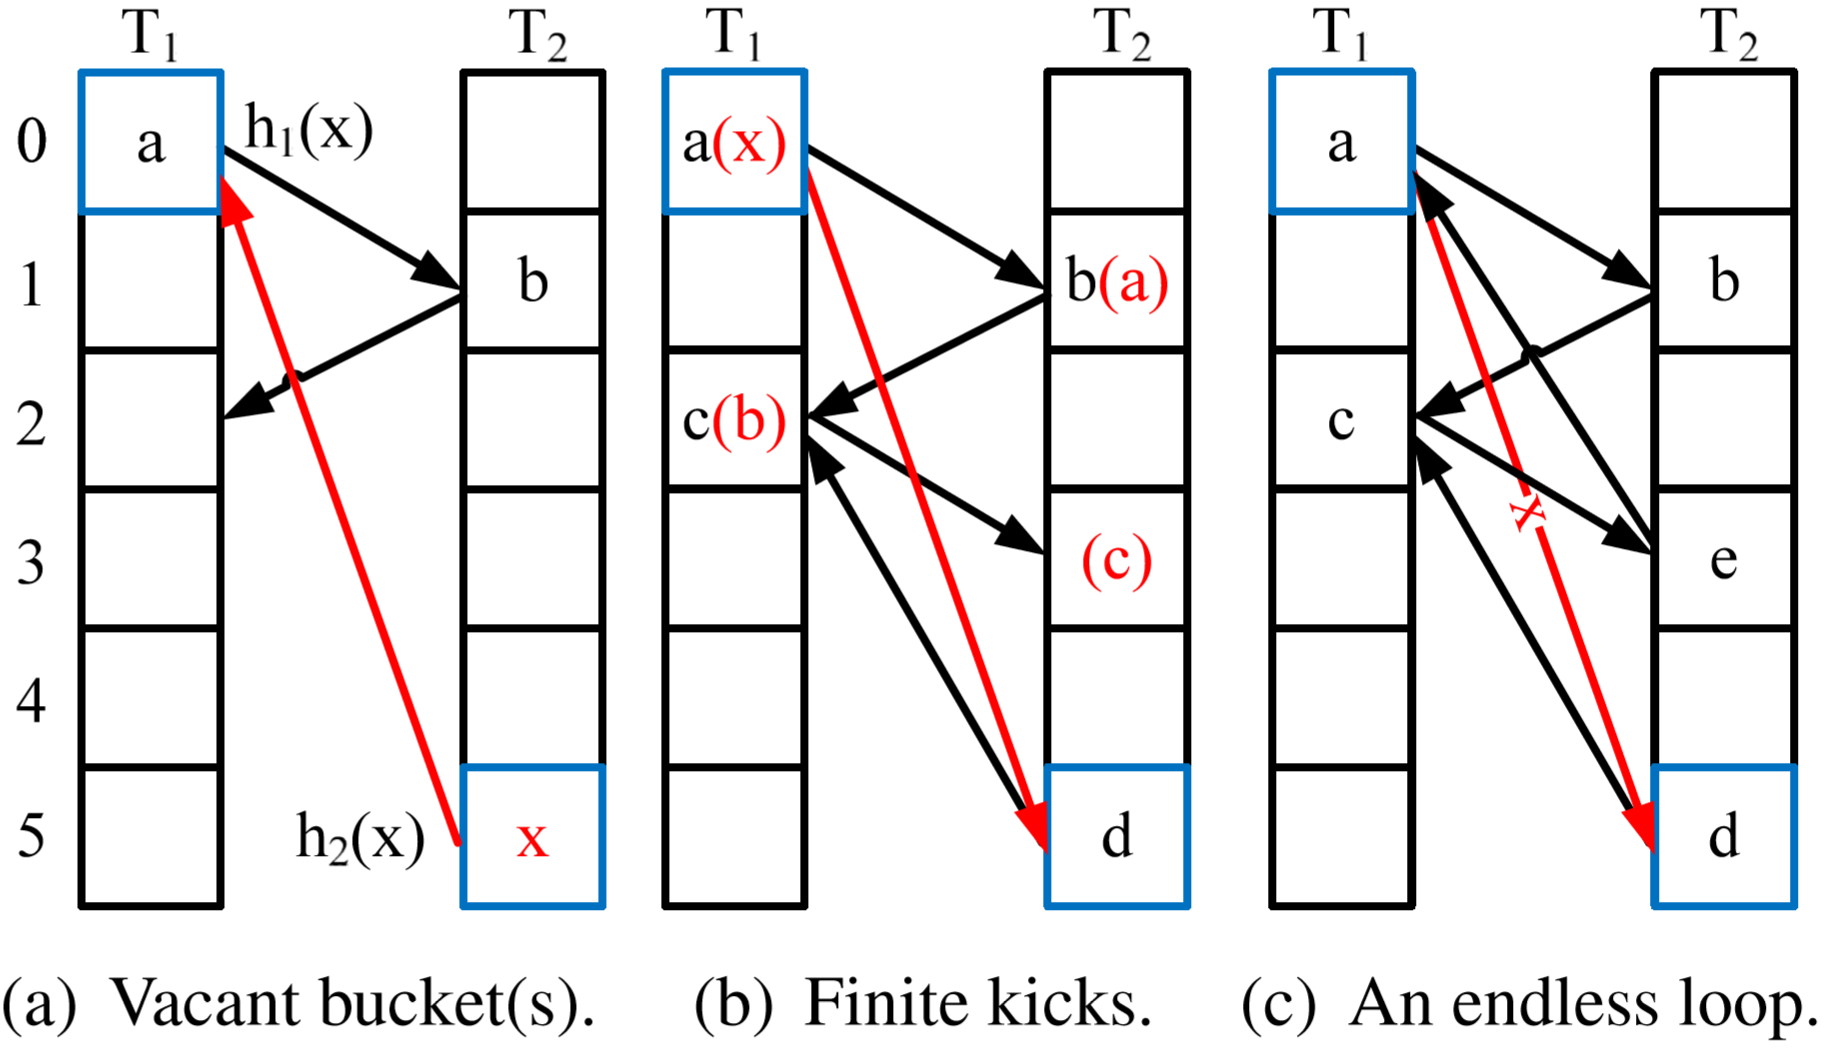
\includegraphics[width=0.65\textwidth]{fig1.png}
    \caption{The standard cuckoo hashing data structure.
    } \label{fig:cuckoo}
\end{figure}

A lookup or delete operation only needs to probes the two candidate buckets of an item, which requires a constant time. For example, to query $x$, we only need to check $T_1[0]$ and $T_2[5]$ as shown in Figure ~\ref{fig:cuckoo}.

If the two hash functions are chosen independently from an appropriate universal hash family, then we can expect to insert all $n$ items successfully with at most $\alpha logn$ kick-out operations for any particluar item with probability $1-O(1/n)$[cuckoo hashing], and $\alpha$ is a sufficiently large constant. Further more, if we limit the number of kick-out operation to $\alpha logn$ before rehashing, then the expected time to insert all $n$ items successfully into the table is $O(n)$, which means the expected insert complexity of the standard cuckoo hashing is also a constant. However, the worst-case insertion time is unpredicatble and should be addressed for real-time storage systems.

\section{Cuckoo Hashing with a Stash}
\label{sec:chs}
TBD.
\section{SmartCuckoo}
\label{sec:smart}
TBD.
\section{Horton Tables}
\label{sec:horton}
TBD.
\section{Conclusion}
\label{sec:conclude}
TBD.

\subsubsection{Sample Heading (Third Level)} Only two levels of
headings should be numbered. Lower level headings remain unnumbered;
they are formatted as run-in headings.

\paragraph{Sample Heading (Fourth Level)}
The contribution should contain no more than four levels of
headings. Table~\ref{tab1} gives a summary of all heading levels.

\begin{table}
\caption{Table captions should be placed above the
tables.}\label{tab1}
\begin{tabular}{|l|l|l|}
\hline
Heading level &  Example & Font size and style\\
\hline
Title (centered) &  {\Large\bfseries Lecture Notes} & 14 point, bold\\
1st-level heading &  {\large\bfseries 1 Introduction} & 12 point, bold\\
2nd-level heading & {\bfseries 2.1 Printing Area} & 10 point, bold\\
3rd-level heading & {\bfseries Run-in Heading in Bold.} Text follows & 10 point, bold\\
4th-level heading & {\itshape Lowest Level Heading.} Text follows & 10 point, italic\\
\hline
\end{tabular}
\end{table}


\noindent Displayed equations are centered and set on a separate
line.
\begin{equation}
x + y = z
\end{equation}
Please try to avoid rasterized images for line-art diagrams and
schemas. Whenever possible, use vector graphics instead (see
Fig.~\ref{fig1}).

\begin{figure}
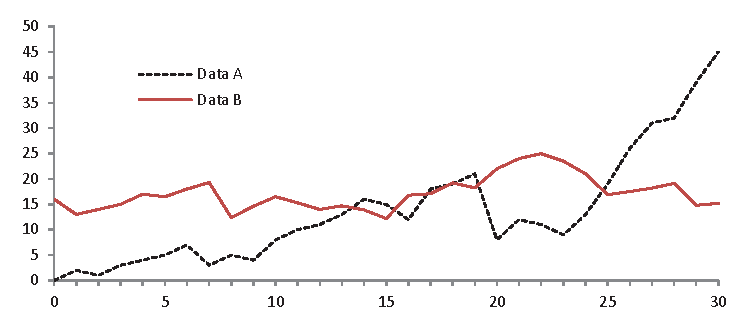
\includegraphics[width=0.5\textwidth]{fig1.eps}
\caption{A figure caption is always placed below the illustration.
Please note that short captions are centered, while long ones are
justified by the macro package automatically.} \label{fig1}
\end{figure}

\begin{theorem}
This is a sample theorem. The run-in heading is set in bold, while
the following text appears in italics. Definitions, lemmas,
propositions, and corollaries are styled the same way.
\end{theorem}
%
% the environments 'definition', 'lemma', 'proposition', 'corollary',
% 'remark', and 'example' are defined in the LLNCS documentclass as well.
%
\begin{proof}
Proofs, examples, and remarks have the initial word in italics,
while the following text appears in normal font.
\end{proof}
For citations of references, we prefer the use of square brackets
and consecutive numbers. Citations using labels or the author/year
convention are also acceptable. The following bibliography provides
a sample reference list with entries for journal
articles~\cite{ref_article1}, an LNCS chapter~\cite{ref_lncs1}, a
book~\cite{ref_book1}, proceedings without editors~\cite{ref_proc1},
and a homepage~\cite{ref_url1}. Multiple citations are grouped
\cite{ref_article1,ref_lncs1,ref_book1},
\cite{ref_article1,ref_book1,ref_proc1,ref_url1}.

\section{SmartCuckoo}
\section{Cuckoo Hashing with a Stash}
\section{Horton Table}
\section{Conclusion}
%
% ---- Bibliography ----
%
% BibTeX users should specify bibliography style 'splncs04'.
% References will then be sorted and formatted in the correct style.
%
% \bibliographystyle{splncs04}
% \bibliography{mybibliography}
%
\begin{thebibliography}{8}
\bibitem{ref_article1}
Author, F.: Article title. Journal \textbf{2}(5), 99--110 (2016)

\bibitem{ref_lncs1}
Author, F., Author, S.: Title of a proceedings paper. In: Editor,
F., Editor, S. (eds.) CONFERENCE 2016, LNCS, vol. 9999, pp. 1--13.
Springer, Heidelberg (2016). \doi{10.10007/1234567890}

\bibitem{ref_book1}
Author, F., Author, S., Author, T.: Book title. 2nd edn. Publisher,
Location (1999)

\bibitem{ref_proc1}
Author, A.-B.: Contribution title. In: 9th International Proceedings
on Proceedings, pp. 1--2. Publisher, Location (2010)

\bibitem{ref_url1}
LNCS Homepage, \url{http://www.springer.com/lncs}. Last accessed 4
Oct 2017
\end{thebibliography}
\end{document}
